
Likewise, the objective of chapter 4 is to describe the researcher's design consideration when developing and testing the prototype. For an overview of the design of the prototype, the researchers considered different computer vision models in classifying the ripeness and bruises together with other algorithms to determine the size of the mango. Likewise, the hardware design was also taken into consideration where the physical design of the conveyor belt was taken into account.

\section{Introduction}
This chapter discusses the design considerations for the mango sorting and grading system, focusing on the technical and engineering decisions required for its development. The design process aims to create a scalable, efficient, and user-friendly system that leverages machine learning for accurate mango classification.

\section{System Architecture}
The system architecture is represented through a block diagram, showcasing modules such as image acquisition, preprocessing, feature extraction, machine learning model, and grading output. Each module is described in detail, emphasizing its role in the overall system. For instance, the image acquisition module uses high-resolution cameras to capture mango images, while the preprocessing module enhances image quality for better feature extraction.

\section{Hardware Considerations}
The hardware components include high-resolution cameras, lighting systems for consistent image capture, and microcontrollers like Raspberry Pi or Arduino for system control, actuators like motors and servo motors to move the mangoes. The choice of hardware is justified based on cost, performance, and compatibility with the software framework.

\subsection{General Prototype Framework}

\subsection{Prototype Block Diagram}

\subsection{Prototype Flowchart}

\subsection{Hardware Specifications}

\subsubsection{Raspberry Pi}
\begin{figure}[!htbp]
	\centering
	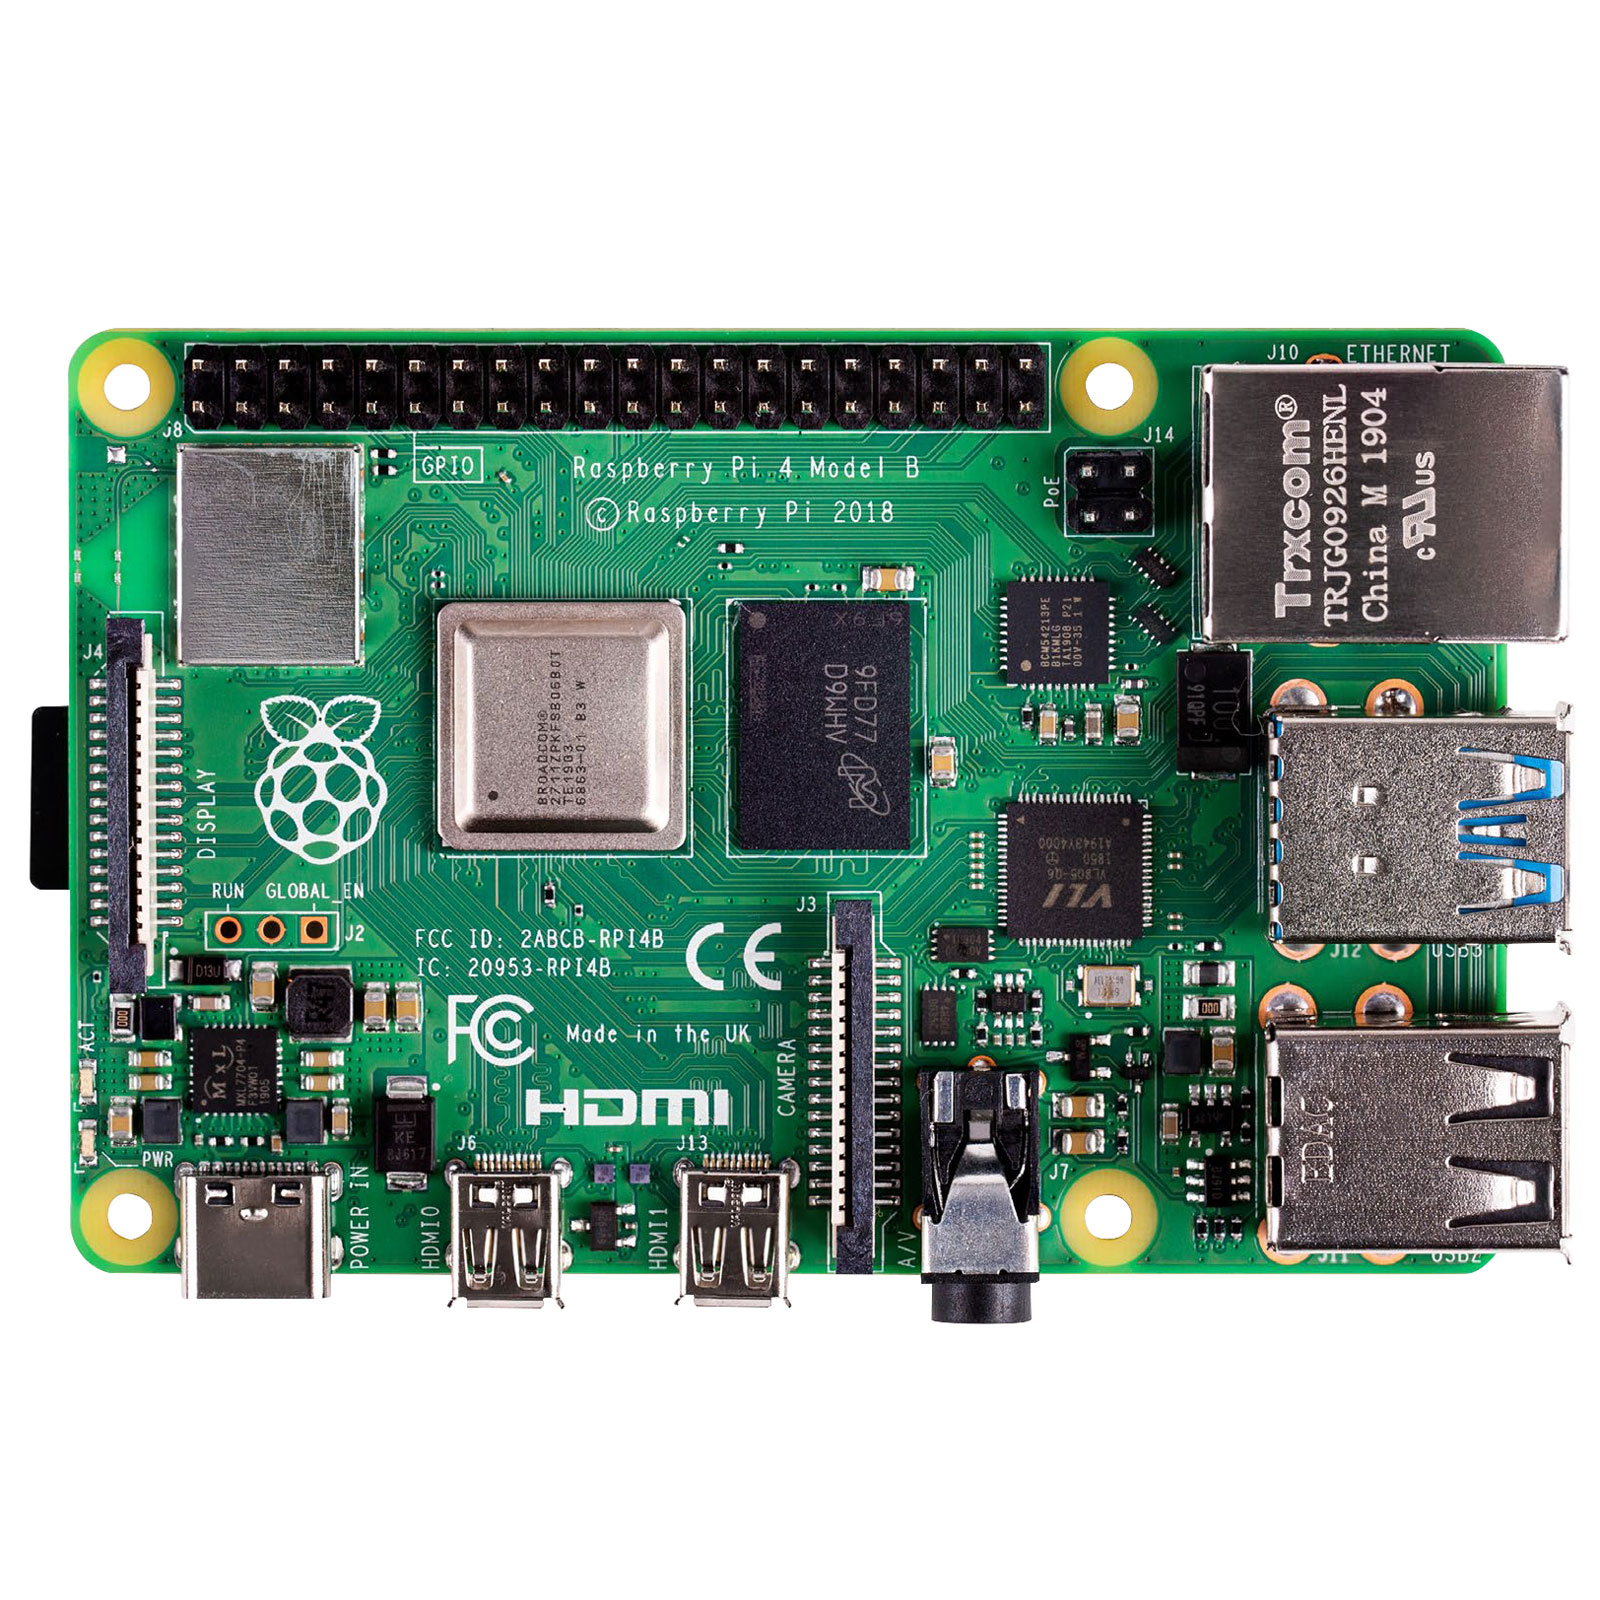
\includegraphics[width=0.5\textwidth]{rpi4b}
	\caption{Raspberry Pi 4 Model B}
	\label{fig:rpi4b_fig}
\end{figure}
The Raspberry Pi 4 Model B is a compact, low-cost computer that serves as the system's main processing unit. 
It is chosen for its balance of performance and affordability, making it suitable for real-time image processing tasks.

\subsubsection{Raspberry Pi Camera}
\begin{figure}[!htbp]
	\centering
	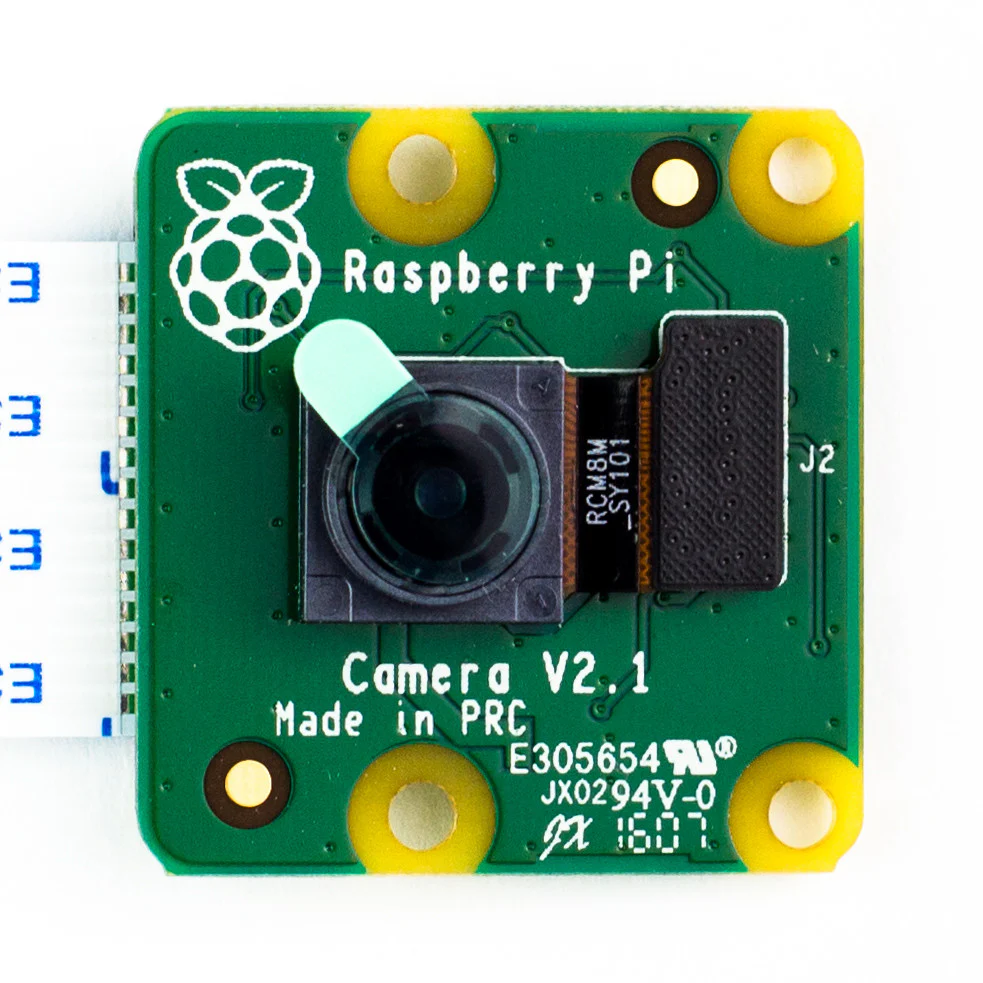
\includegraphics[width=0.5\textwidth]{rpi_cam}
	\caption{Raspberry Pi Camera Module Version 2}
	\label{fig:rpi_cam_fig}
\end{figure}

\subsubsection{DC Motor}
\begin{figure}[!htbp]
	\centering
	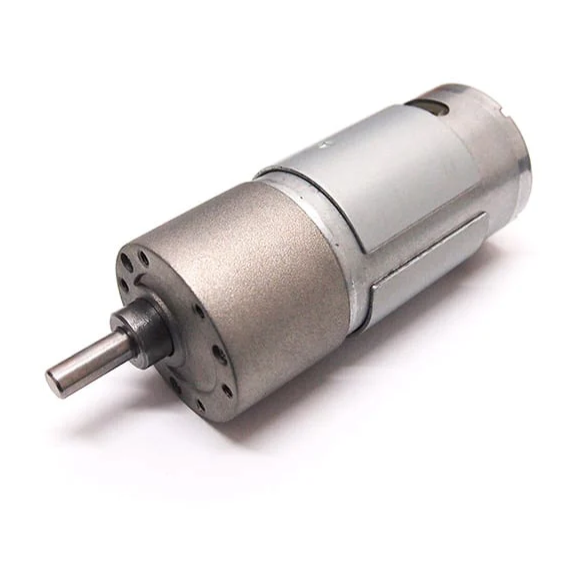
\includegraphics[width=0.5\textwidth]{dc_motor}
	\caption{12 Volt DC Gear Motor}
	\label{fig:dc_motor_fig}
\end{figure}

\subsubsection{MicroSD Card}
\begin{figure}[!htbp]
	\centering
	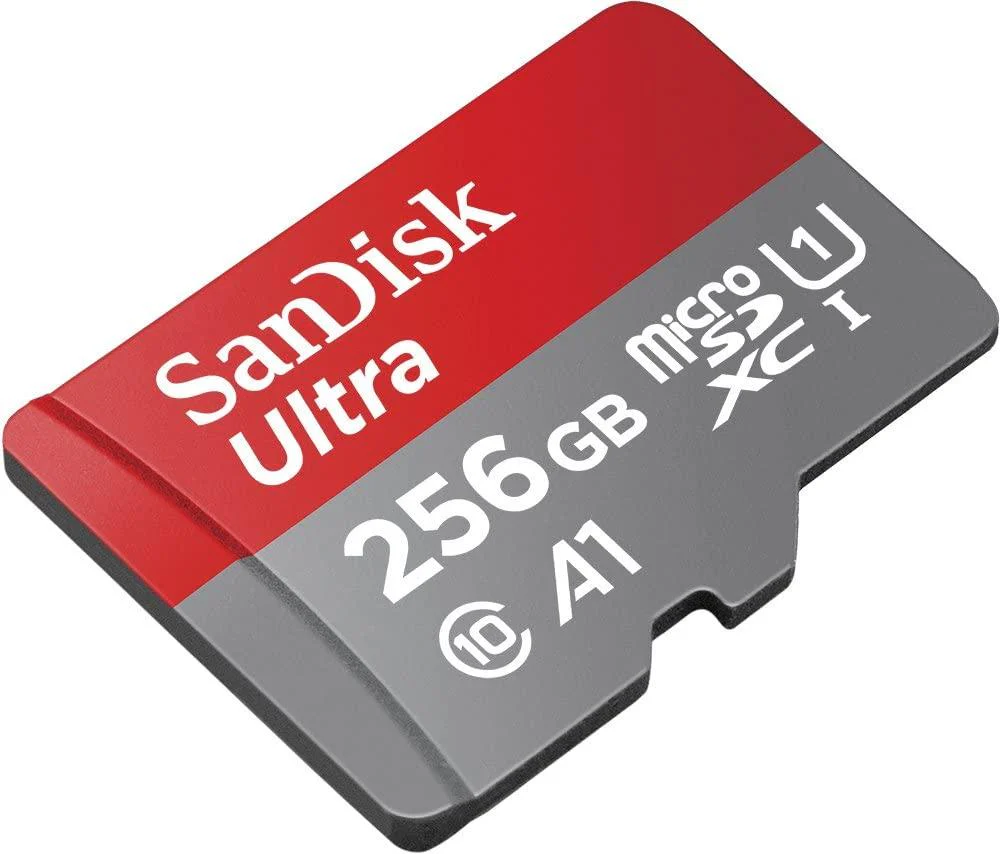
\includegraphics[width=0.5\textwidth]{sdCard}
	\caption{SanDisk Ultra MicroSD Card}
	\label{fig:sdCard_fig}
\end{figure}


\subsubsection{LED Lights}
\gls{led} lights are used to provide consistent lighting for image capture, ensuring accurate color representation and feature extraction.

\subsubsection{Power Supply}
\begin{figure}[!htbp]
	\centering
	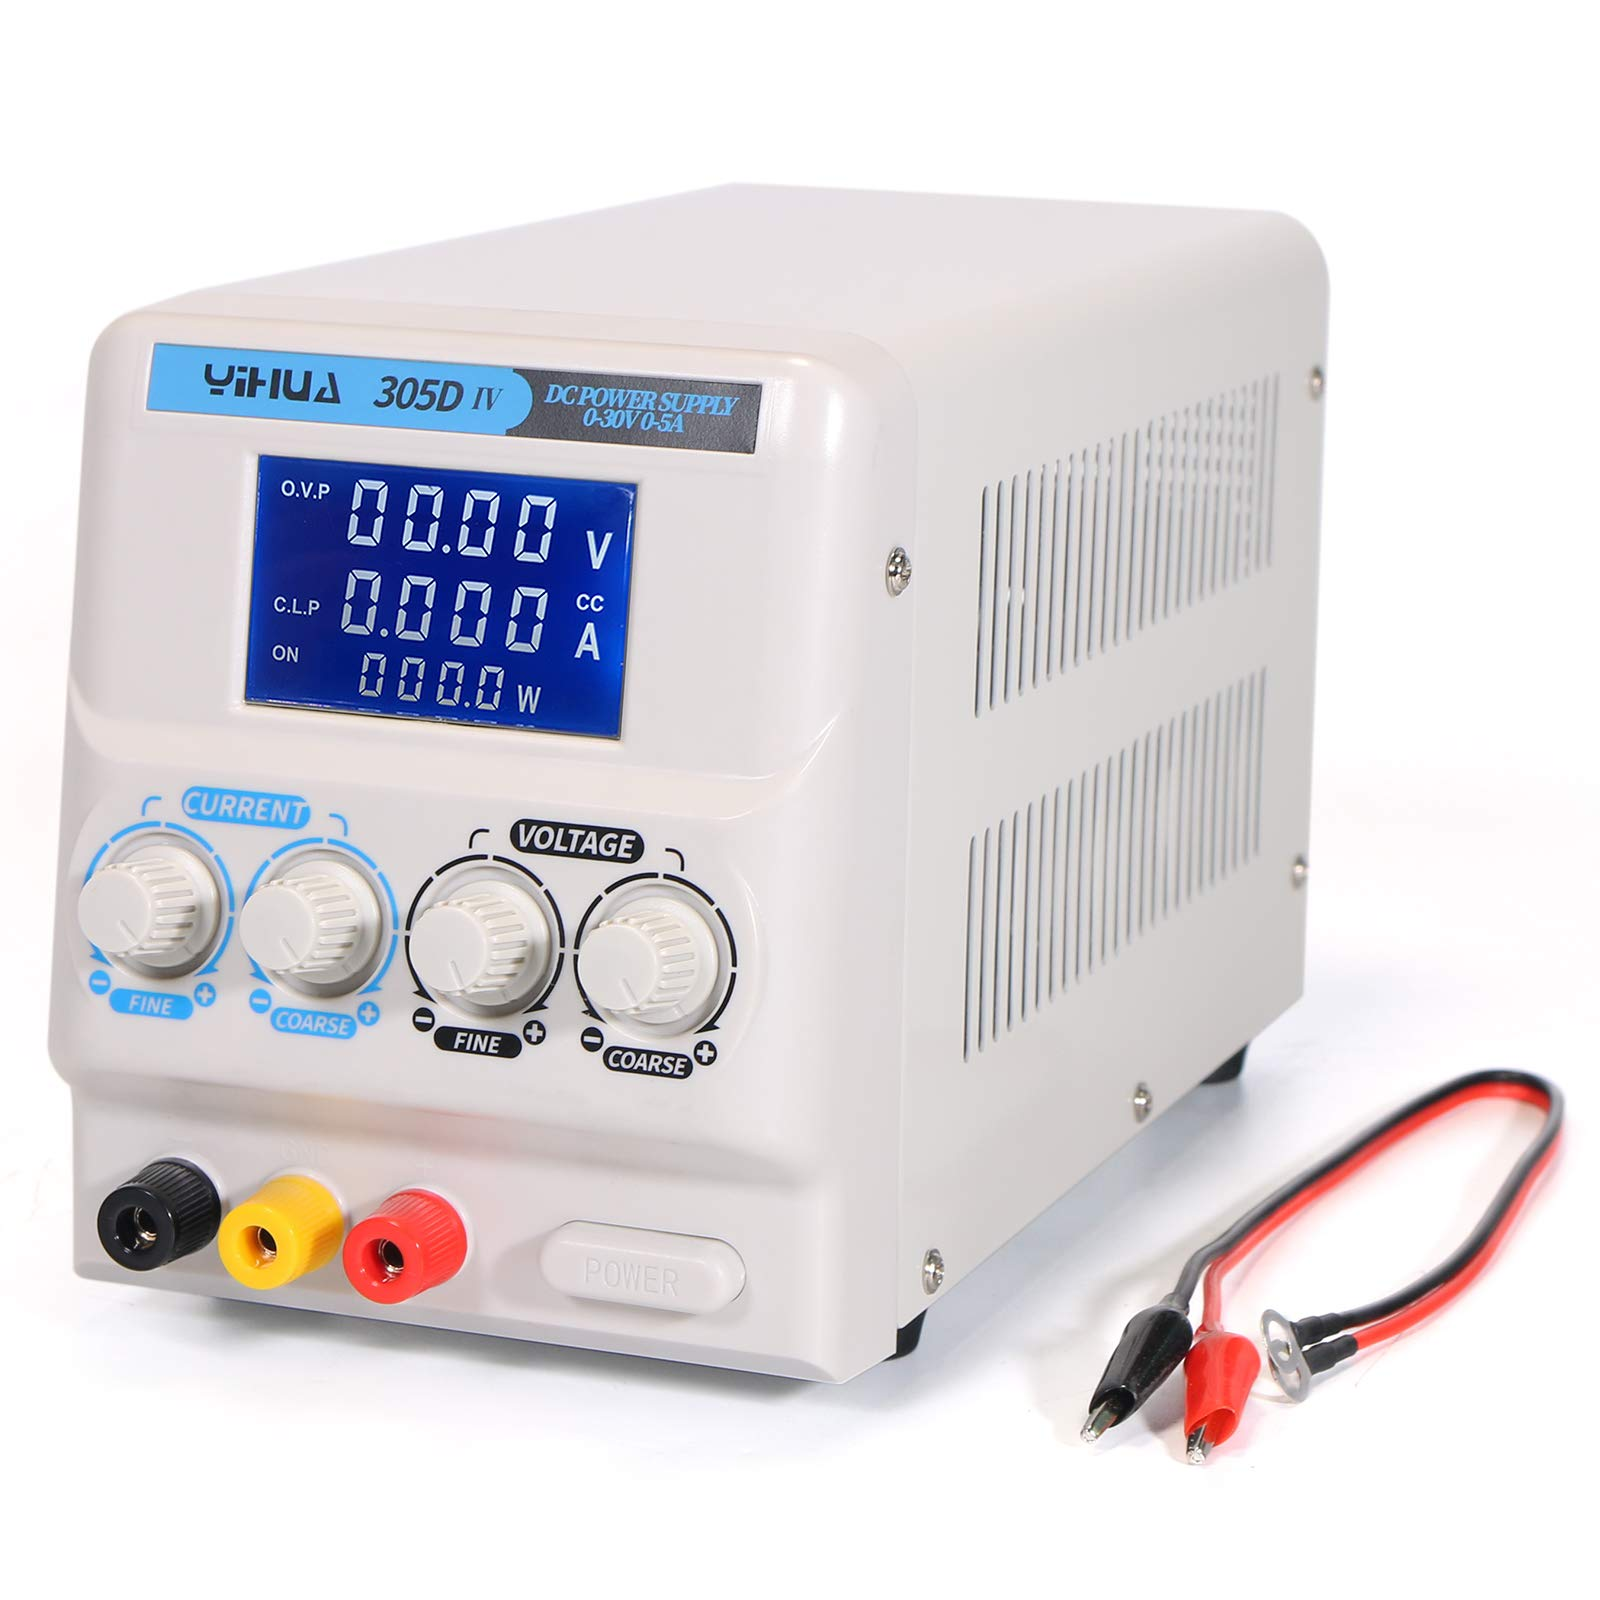
\includegraphics[width=0.5\textwidth]{Power_Supply}
	\caption{Bench Power Supply}
	\label{fig:Power_Supply_fig}
\end{figure}


\subsubsection{4 Channel Relay Module}
\begin{figure}[!htbp]
	\centering
	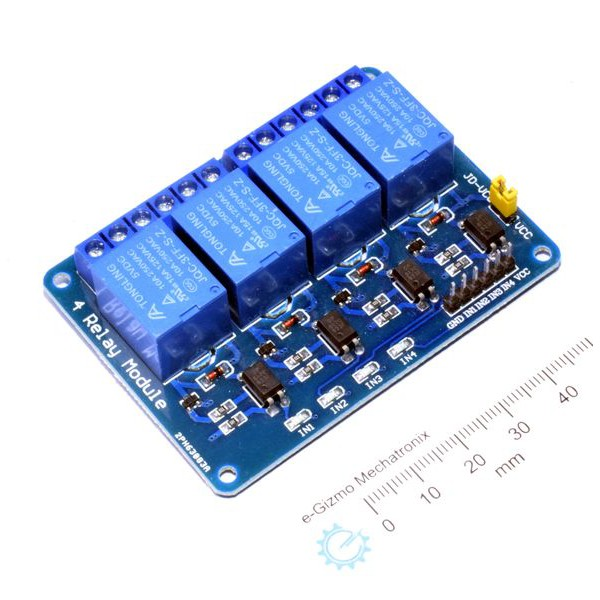
\includegraphics[width=0.5\textwidth]{relay_module}
	\caption{4 Channel Relay Module}
	\label{fig:relay_module_fig}
\end{figure}


\section{Software Considerations}
The software stack includes Python for programming PyTorch for machine learning and OpenCV for image processing. These tools are selected for their robustness, ease of use, and extensive community support, ensuring efficient system development.

\subsection{PyTorch}

\subsection{OpenCV}

\subsection{Tkinter}

\subsection{CustomTkinter}

\section{Security and Reliability Considerations}
Potential vulnerabilities, such as data corruption during image capture, are addressed through redundancy and error-checking mechanisms. Reliability is ensured by implementing fault-tolerant designs and rigorous testing protocols.

\section{Scalability and Efficiency Considerations}
The system is designed to handle large volumes of mangoes by optimizing the machine learning model and using parallel processing techniques. Efficiency is improved through techniques like model quantization and hardware acceleration.

\section{User Interface}
A \gls{ui} is designed to display grading results, system status. Wireframes illustrate the layout, ensuring usability and accessibility for operators. 
Likewise, a \gls{gui} is also used to allow users to customize the system's grading priorities.

\section{Constraints and Limitations}
Challenges include variations in mango appearance due to lighting and environmental factors. Trade-offs are made between model complexity and real-time performance to balance accuracy and speed.

\section{Technical Standards}
The system adheres to industry standards for image processing and machine learning, ensuring compatibility and interoperability with other systems.

\section{Prototyping and Simulation}
Prototypes are developed using tools like MATLAB and Simulink to simulate the system’s performance. These simulations help identify design flaws and optimize the system before deployment.,

\section{Design Validation}
The design is validated through testing, including unit testing of individual modules and integration testing of the entire system. Peer reviews and iterative improvements ensure the system meets the desired performance metrics.

\section{Summary}
This chapter outlined the key design considerations, including system architecture, hardware and software choices, and validation methods. These decisions are critical for developing a reliable and efficient mango sorting and grading system.

